\section{Introduction}
\label{sec:intro}


\todo{To be written}


\myparagraph{Motivation} The attacker can easily change system configurations (i.e., install root certificates), alter the user's transaction, or manipulate the user by showing false information on the screen. Figure~\ref{fig:motivation} provides four such cases where the secrecy and the integrity of the input and output data are crucial. Effectively the primary motivation of this work is to build an efficient and effective \emph{trusted path} solution that provides the highest form of security regarding integrity and privacy. 

Based on these examples we list the security properties that we want to provide in our proposed solution. We now discuss these security properties and corresponds them with the motivating example.

\begin{mylist}
  \item \textbf{Input integrity and privacy.} Input security can be classified into two subfeatures, namely input integrity and input privacy. In a case where the user provides input to a remote safety-critical system, input integrity is a crucial property that ensures that the command from the user reaches to the remote end-point without any modification by the malicious host system. Case 1 in Figure~\ref{fig:motivation} is a concrete example where input integrity is critical for the application to be work properly. Input privacy is required if the malicious host wants to steal the sensitive information from the user. This involves the credentials for various web-service, financial information such as the credit card number, choice of the vote in the e-voting system. Cases 2, 3,and 4 in Figure~\ref{fig:motivation} are the example where input privacy is needed.
  \item \textbf{Output Integrity and privacy.} Similar to the input security, output security has two aspects: output integrity and privacy. Output integrity is a critical component to ensure a secure display. This involves data coming from remote safety-critical devices, medical implants, financial data such as the bitcoin address, candidate list in the e-voting portal, etc. Cases 1, 2, and 3 in Figure~\ref{fig:motivation} are the potential scenarios where output integrity property is desirable. In many application scenarios, output privacy is required where the data sent from the remote end-point is privacy sensitive. Such includes the web credentials, candidate preference data in the e-voting, the private key of the bitcoin wallet, etc. Example scenarios 2, 3 and 4 in Figure~\ref{fig:motivation} require output privacy. Additionally, we identify a sub category of output intergrity  that we call the \emph{integrity of the UI} where that ensures that the host system renders the UI in faithful way, i.e., the host system does nor modify the UI elements on the screen to trick the user into proving any additional information that may be sensitive.
  
  \item \textbf{Sandboxed activity.} We define activity analogously to the user intention which is privacy sensitive in many application scenarios. One such concrete example is e-voting where voting privacy is of uttermost importance. Even if there is a system in place that provides input privacy, merely the fact that the user may hover her mouse over some candidates may reveal her candidate preference. Activity privacy is application specific, and in most of the case, it dynamically preserves a part of the scene where the user activity is oblivious to the compromised host. 
  \item\textbf{Low-TCB auxiliary device.} The above security properties are needed to be achieved without assuming any other primitives such as trusted execution environments, trusted hypervisor etc. Instead we opt for a very low TCB embedded auxiliary device that aids the users to achieve all the security properties without compromising usability of the system. 
\end{mylist}

\begin{figure}[t]
\centering
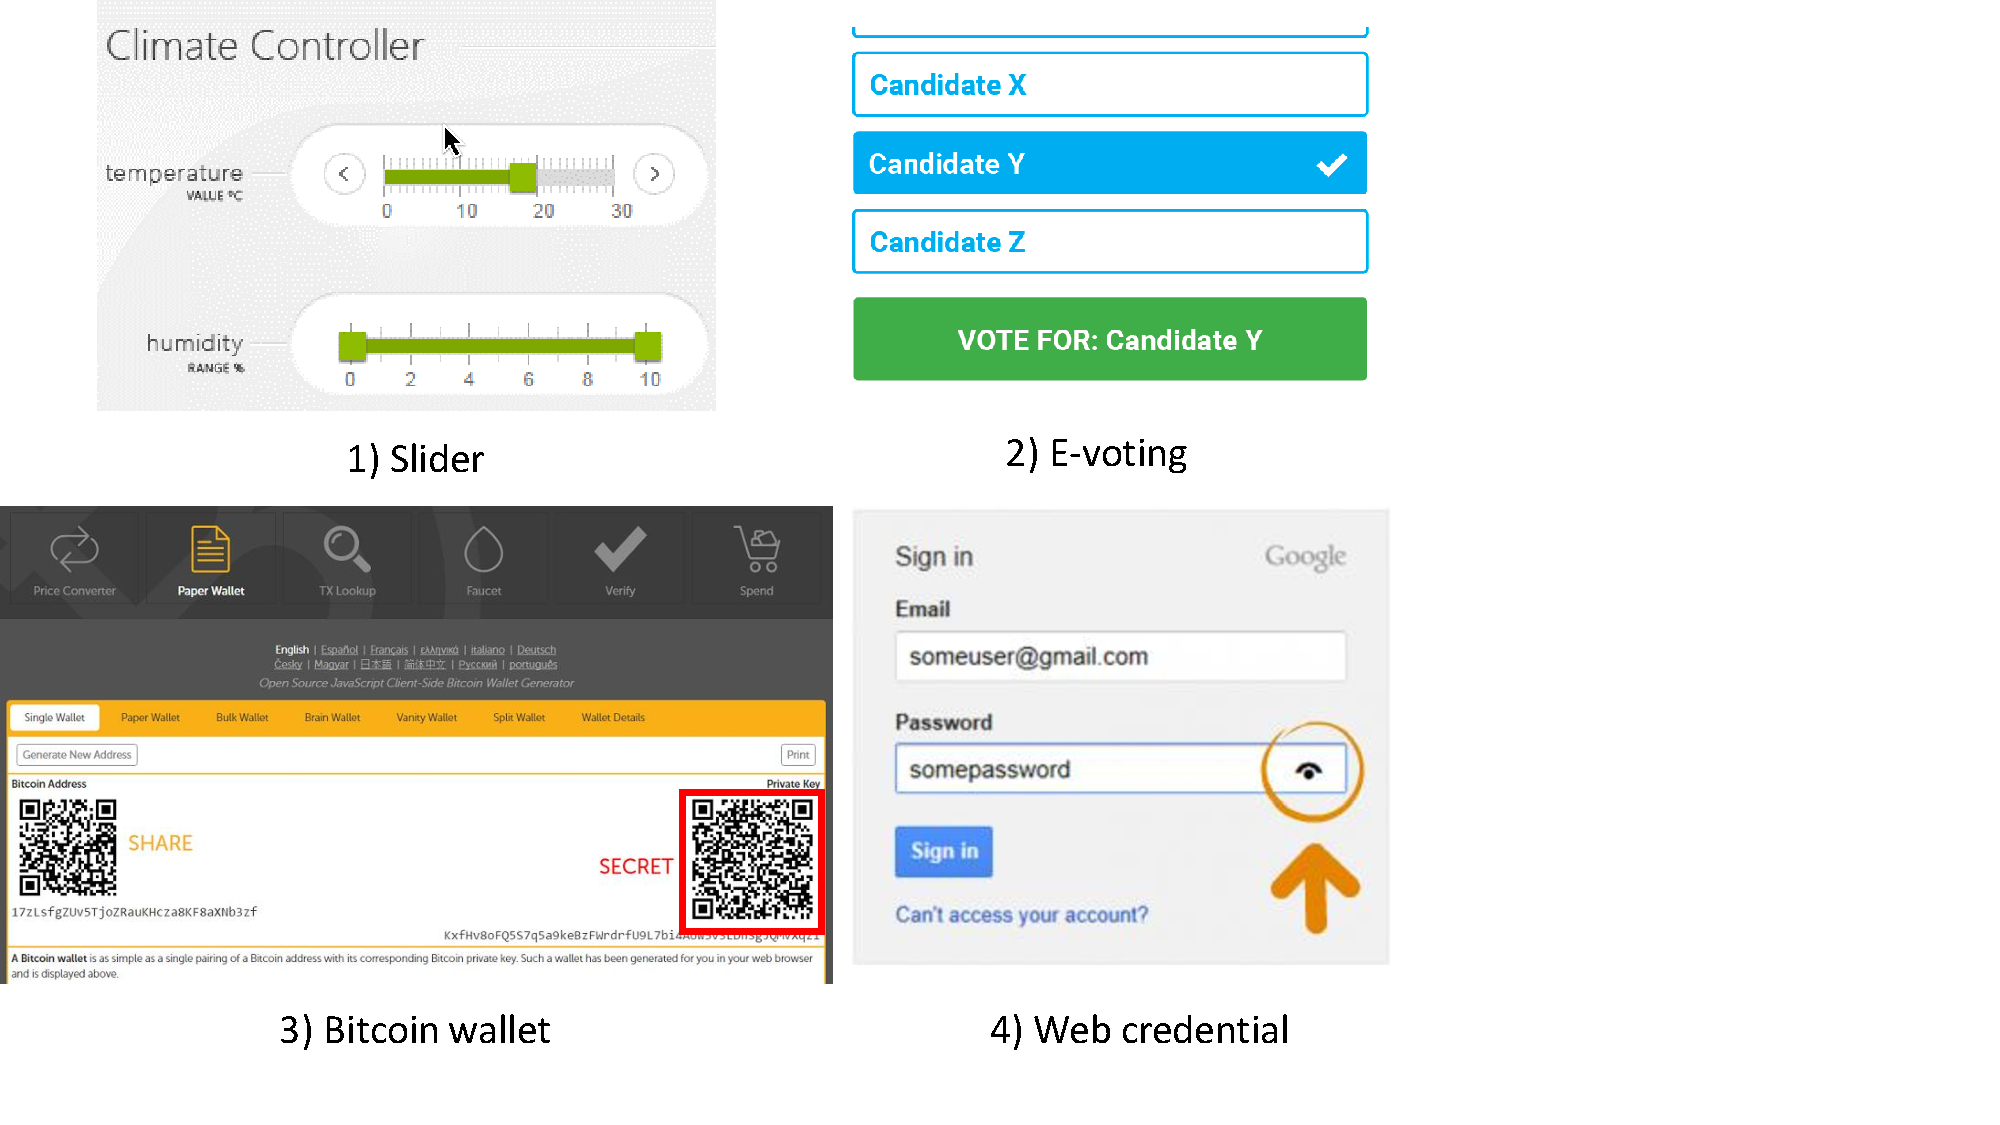
\includegraphics[trim={0 1cm 10cm 0}, clip, width=\linewidth]{motivation.pdf}
\caption{\textbf{Motivating examples.} 1) Pointer based UI elements that sets parameters to remote safety-critical device, 2) E-voting where the voting privacy and integrity is critical, 3) Financial transactions such as bitcoin wallet that shows sensitive information such as the user's private key and 4) web applications that provide an option for the user to reveal credentials.}
\label{fig:motivation}
\centering
\end{figure}

\myparagraph{Contributions}
\begin{mybullet}
  \item Track the mouse pointer and key stroke on the screen to understand user intention.
  \item Understand the application context from the frames captured from the HDMI stream.
  \item Private input activity of the user.
  \item Fully end-to-end IO (input and output) privacy and integrity.
  \item Could be integrated into the graphics card driver making them as an isolated IO environment,
  \item Easy to setup (no hypervisors, modifications in drivers or OS, no extra application or TEEs), the device is installed between the host and the display, no need to modify websites, or install any application to the host system.
\end{mybullet}